%================================================================================
%=============================== DOCUMENT SETUP =================================
%================================================================================

%\documentclass[lang=ngerman,inputenc=utf8,fontsize=10pt]{ldvarticle}
\documentclass[lang=ngerman,inputenc=utf8,fontsize=10pt]{ldvarticle}
%PACKAGES

\usepackage{parskip}
\usepackage{subfigure}
\usepackage{ifthen}
\usepackage{comment}
\usepackage{color}
\usepackage{colortbl}
\usepackage{soul}
\usepackage{tikz}
\usetikzlibrary{shapes,arrows}
\usepackage{tabularx}
\usepackage{lipsum}
\usepackage{pgfgantt}
\usepackage{amsmath}

\usepackage{color}

\usepackage[backend=biber,style=ieee,
doi=false,isbn=false,url=false,eprint=false]{biblatex}
\addbibresource{Relevant.bib}

\definecolor{lightgray}{rgb}{0.75,0.75,0.75}


\usepackage{tikz}
\usetikzlibrary{calc}
\usetikzlibrary{calendar}

\newcommand{\countweek}{\ifdate{equals=01-01}{\setcounter{weekcounter}{0}}{} \ifdate{Thursday}{\stepcounter{weekcounter}}{}}

% GanttHeader setups some parameters for the rest of the diagram
% #1 startdate
% #2 enddate
% #3 with of 
\def\GanttHeader#1#2#3{%
\newcounter{weeks}
\newcounter{weekcounter}
\def\withdes{3cm}
\def\hrows{0.4cm}
%get number of weeks
\calendar [dates=#1 to #2,day code={},
execute after day scope=
{\ifdate{Thursday}{\stepcounter{weeks}}{}}];

%get the currend KW
\calendar [dates=2021-01-01 to #1+-1,day code={},
execute after day scope=
{\countweek}];

%calcualate the shifts
\pgfmathsetmacro{\dayshift}{(\textwidth-\withdes)/(\theweeks*7)}

\tikzstyle{every day}=[anchor=mid]
\calendar [dates=#1 to #2,day code={},
execute after day scope=
{\countweek \ifdate{Thursday}{\node {\tiny\textbf{\theweekcounter}};}{} 
	\ifdate{Sunday}{\draw[thick] (0,-0.5*\hrows) -- +(0,\hrows);}{} 
	\ifdate{day of month=15}{\node[] at (0,\hrows) {\small{\tikzmonthtext}};}{} 
	\ifdate{day of month=1}{\draw[thick] (0,0.5*\hrows) -- +(0,\hrows);}{}
	\pgftransformxshift{\dayshift}}] 
at (\withdes,0); %set position

%setup descriptions
\draw[very thick] (0,0.5*\hrows) rectangle +(\withdes, \hrows);
\draw[very thick] (0,-0.5*\hrows) rectangle +(\withdes, \hrows);
\draw[very thick] (\withdes,0.5*\hrows) rectangle +(\textwidth-\withdes, \hrows);
\draw[very thick] (\withdes,-0.5*\hrows) rectangle +(\textwidth-\withdes, \hrows);
\node[] at (0.5*\withdes,\hrows) {\small{\textbf{Month}}};
\node[] at (0.5*\withdes,0) {\small{\textbf{Week}}};
}


% This macro adds a task to the diagram
% #1 Row of the Task
% #2 Task's name
% #3 Starting Week
% #4 Duration (Weeks)
\def\Task#1#2#3#4{%
\begin{scope}[shift={(0,-0.2*\hrows-#1*\hrows)}]
  \filldraw[fill=black!20,thick] (0,-0.5*\hrows) rectangle +(\textwidth, \hrows);
\node[anchor=west] at (1mm,0) {\small{\textbf{#2}}};
 \filldraw[color=red] (\dayshift*7*#3+\withdes,-0.45*\hrows) rectangle +(\dayshift*7*#4+0cm,0.9*\hrows);
  \foreach \x in {0,...,\theweeks} {
    \draw[thick] (\dayshift*7*\x+\withdes,-0.5*\hrows) -- +(0,\hrows);
}
\end{scope}
}







\usetikzlibrary{matrix}


\DeclareMathOperator{\vect}{vec}

%================================================================================
%================================= TITLE PAGE ===================================
%================================================================================

\title{Combining Matrix Representations for Structured Approximation of Neural Network Weight Matrices}
\subtitle{Projectplan}
\author{Stepahn Nüßlein}

\date{\today}

\begin{document}


	\maketitle
	\thispagestyle{empty}
	\vspace*{2cm}
	\hrule

\section*{Motivation}

As the matrices for fully connected layers get larger the evaluation of the neuronal nets get computationally more expensive. This is often problematic as the computational resources are a limiting factor, especially on embedded or mobile systems.
Therefore different approaches to reduce the computational cost are being explored.

A possible representation are Sequentially Semiseperable Matrices. These have a certain underling structure.
The matrices in Neuronal Networks do not necessarily have the same underling structure.
Even if the Matrix is close the to a Sequentially Semiseperable Matrix the structural Parameters might not be know.

To increase the number of Matrices that can be represented we allow combinations of Sequentially Semiseperable Matrices.
This means that a Matrix can also be represented as as sum of multiple Sequentially Semiseperable Matricies.

To represent the matrices, an algorithm to derive the representation is needed.
	%\item Both approxiamtion of Matrix in some Norm ($\|\|_F$,$\|\|_1$,$\|\|_\infty$ or similar) also Accuracy on Data set




\vspace*{1cm}
\hrule

\newpage

\section{Project Description}

\subsection*{Goals}

\begin{itemize}

	\item\textbf{Matrix approximation with reduced cost} Find a Matrix approximation. This requires a formal definition, as well as a reference implementation.
	\item\textbf{Algorithm to construct said approximation} Development of an algorithm to calculate the approximation. Also implement an reference implementation
	\item\textbf{Theoretical description of description} Compile the theoretical properties that can be derived.
	\item\textbf{Evaluate approximation in practical examples} Evaluate the performance on weight matrices from pretrained models form Pytorch. This includes the behaviour of the approximation algorithm, the computational cost as well as the performance of the neuronal net
\end{itemize}





\subsection*{Approach}

These assumptions and properties are underlying the idea:
\begin{itemize}
	\item Matrices in fully connected layers often have full rank. This means that a rank reduction is not easily possible (with some caveats, as it is not certain that this is the relevant ingredient) \cite{martin_implicit_2018}
	\item To get the optimal trade of between accuracy and cost it should be possible to adapt the accuracy of the approximation by changing hyper parameters of the approximation.
\end{itemize}

By fixing the input and output Dimensions of an a State-Space representation we fix an segmentation of the representable matrices.
The matrices in a neuronal net might not have an underling structure that can be represented with the resulting segmentation.

Therefore it might be interesting if the Matrices in an neural net can be better described with a sum of Matrices.

A similar representation with products of SSS Representations with non matching output and input dimensions might also be possible, but is harder to describe.


\subsubsection*{Next steps}

One prerequisite is finding appropriate segmentation of the Matrix. This either includes finding a existing way of finding a segmentation and implementing it.
Or coming up with a an algorithm to segment a matrix.

This would require segmenting a matrix into different areas that are similar to a low rank matrix. This also has to take into account that SSS matrices have many overlaying areas with low rank.

Furthermore an Algorithm to combine different SSS Representations in a adequate way is needed.

\subsubsection*{Theoretical considerations}
To support this by theory it might be interesting to build some theoretical background on the decomposition.
A first step is having a look at the formulas from state space arithmetic. While deriving closed form representations for cases with non matching dimensions might not be possible, it might give some insight.

It should be tested if the SSS Matrices can be represented as a manifold. This might allow some theoretical results.
Additionally it should be tested if it is possible to describe more complex objects like sums.
This might make it possible to show something on how "dense" the representable matrices are in the space of all matrices.



\subsubsection*{Computational cost}
The computational cost of evaluation a matrix vector product is determined by the number of parameters.
For the SSS structure the number of multiplications is equal to the number of nonzero entries in the A,B,C and D matrices. These depend on the dimensions of the input and output and on the number of states.

As we like to minimize the computational cost it will be necessary to setup a detailed formula for the computational cost depending on the structural parameter.


\subsubsection*{Properties}
The computational stability of the resulting algorithm should be tested numerically. This might be for further interest if it the evaluation is done on an 32-bit architecture.


\subsubsection*{Calculation of Representation}
There are two possible ideas to get the wanted representation:

\paragraph{Optimization Problem}
Convert the given properties into manifolds and objective functions and use optimization techniques.
This might be easier to define, but will possibly result in a problem with a very high number of dimensions. Maybe it is possible to express it as some standard problem, then it would be possible to use standard solvers and use existing guarantees and runtime estimates.

\paragraph{Iterative Methods}
Use an approach similar to Matching pursuit. Here the dictionary $D$ would be a subset of all Sequentially Semiseperable Matrices. This requires some description of a qasi-inner-product and an way to find an approximation of the closest element in $D$.
As $D$ will have infinitely many dimensions, this might be quite involved.



\section{Workpackages}

\begin{itemize}
	\item \textbf{Recherche:}
	\begin{itemize}
			\item \textbf{Existing Decompositions:} Low Rank+Sparse, Multiscale Low rank \cite{chandrasekaran_sparse_2009,ong_beyond_2016,yu_compressing_2017}
			\item \textbf{Sparsity:} Appropriate Sparsity Measures \cite{ulfarsson_sparse_2015,parekh_improved_2017}
			\item \textbf{Existing Algorithms:} Look into the structure of related algorithms
		\end{itemize}
	\item \textbf{Evaluierung:} Analyse der bisherigen Recherce
		\begin{itemize}
			\item \textbf{Auswahl:} choose appropriate assumptions
			\item \textbf{Theoretical considerations:} Try the theoretical questiosn outlined above.
		\end{itemize}
	\item \textbf{Implementierung:} Implement Algorithm
		\begin{itemize}
			\item \textbf{Implement Algorithm(s):} Based on previous exploration choose algorithm to construct the representation. If uncertain implement two different approaches and try them on examples.
			\item \textbf{Generate Tests:} Generate Testsdata and pipeline to test them, including meta-analysis (speed of convergence...)
		\end{itemize}
	\item \textbf{Analyse:} Entwurf und Durchführung praxisnaher Tests
		\begin{itemize}
			\item \textbf{Setup Test}
			\item \textbf{Evaluation I:} Evaluation on tailor-made examples: Combiantion of Sequentially Semiseperable Matricies %(I think we need more than $\min(n,m)$ rank sub matrices until the standard SVD not be able to recover the structure?, but even then it might be interesting, as we can reduce the computations)
			\item \textbf{Evaluation II:} Random matrices with different parameters
			\item \textbf{Evaluation III:} Evaluation on AI matrices
		\end{itemize}
	\item \textbf{Auswertung und Diskussion:} Ergebnisse zusammentragen und vergleichen
		\begin{itemize}
			\item \textbf{Revisiting the Theory:} Explanations for experienced behavior?
			\item \textbf{Description of Performance:} Beschreibung der durchgeführten Tests und Visualisierung der Ergebnisse
			\item \textbf{Diskussion:} Auswertung der Ergebnisse und kritische Betrachtung des Nutzens für das Gesamtsystem
		\end{itemize}
	\item \textbf{Ausarbeitung:} Abschließende schriftliche Darstellung der durchgeführten Arbeiten
\end{itemize}

\section{Time Table}



	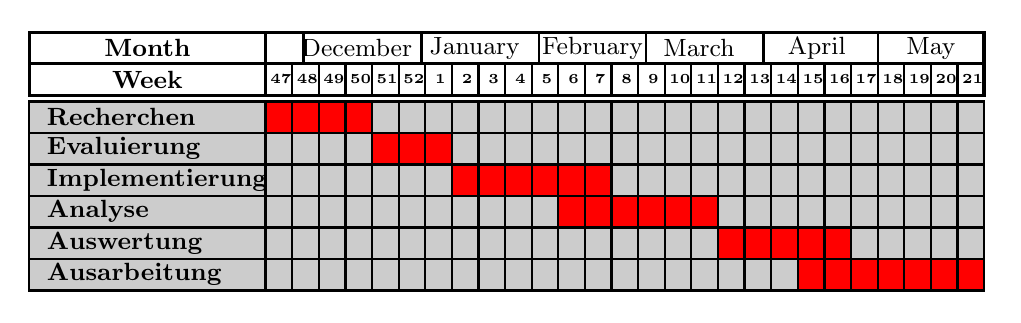
\begin{tikzpicture}
	\GanttHeader{2021-11-21}{2022-05-29}{\textwidth}


	\Task{1}{Recherchen}{0}{4}
	\Task{2}{Evaluierung}{4}{3}
	\Task{3}{Implementierung}{7}{6}
	\Task{4}{Analyse}{11}{6}
	\Task{5}{Auswertung}{17}{5}
	\Task{6}{Ausarbeitung}{20}{7}
	\end{tikzpicture}






\section{Risk Analysis}

Computation effort might not be lower than the effort for regular matrix vector product.
\newline\textbf{Likelihood:} Risk is hard to determine upfront as it depends on how many fast the approximation converges.
\newline\textbf{Mitigation:} Test practical examples at an early stage of the thesis and.

Unable to find an appropriate algorithm
\newline\textbf{Likelihood:} Quite likely as it is a very underdetermined problem with many parameters
\newline\textbf{Mitigation:} use more computation-time, reduction of degrees of freedom by requiring some artificial condition (e.g. set the structure of the submatrices)


\printbibliography

\end{document}
